\documentclass[8pt,a4paper]{extarticle}
\usepackage[utf8]{inputenc}
\usepackage[T1]{fontenc}
\usepackage[romanian]{babel}
\usepackage[margin=0.7cm,columnsep=0.45cm]{geometry}
\usepackage{amsmath,amssymb,mathtools}
\usepackage{enumitem}
\usepackage{titlesec}
\usepackage{multicol}
\usepackage{tikz}
\usepackage{array}
\usetikzlibrary{arrows.meta}
\usepackage[most]{tcolorbox}
\usepackage[colorlinks=true,linkcolor=red!55!black,urlcolor=red!55!black]{hyperref}

\newtcolorbox{keyeq}{colback=red!6,colframe=red!65!black,boxrule=0.6pt,arc=1.5pt,
  left=3pt,right=3pt,top=0.5pt,bottom=0.5pt,breakable}

\setlist{nosep, topsep=0pt, itemsep=0pt, leftmargin=1.1em}
\titleformat{\section}{\normalfont\bfseries}{\thesection.}{0.4em}{}
\titleformat{\subsection}{\normalfont\bfseries}{\alph{subsection})}{0.4em}{}
\titlespacing*{\section}{0pt}{2pt}{1pt}
\titlespacing*{\subsection}{0pt}{1pt}{0.5pt}
\renewcommand{\baselinestretch}{0.9}
\setlength{\parindent}{0pt}
\setlength{\parskip}{1.5pt}
\abovedisplayskip=2pt plus 1pt minus 1pt
\belowdisplayskip=2pt plus 1pt minus 1pt
\abovedisplayshortskip=1pt plus 1pt
\belowdisplayshortskip=1pt plus 1pt
\pagestyle{empty}

\begin{document}
\begin{center}
{\large\bfseries Formule rezolvare TS2 --- 2026}
\end{center}
\vspace{-0.3cm}

\begin{multicols}{2}
\footnotesize

\section{Model de stare}

\subsection{Model canonic controlabil}
$$G(s)=\dfrac{b_1s+b_0}{s^2+a_1s+a_0}$$
\begin{keyeq}
$$A=\begin{pmatrix}0&1\\-a_0&-a_1\end{pmatrix},\ B=\begin{pmatrix}0\\1\end{pmatrix}$$
$$C=\begin{pmatrix}b_0&b_1\end{pmatrix},\ D=0$$
\end{keyeq}

\subsection{Model de stare (general) + schemă bloc}
$$\dot x = Ax+Bu \qquad y = Cx+Du$$
Schema bloc: integratoare + reacții după $A,B,C$ (vezi PDF rezumat).

\subsection{Răspuns la treaptă unitară}
$$U(s)=\frac1s,\qquad Y(s)=G_0(s)U(s)$$
Desfaci $Y(s)$ în fracții simple (partial fraction), apoi:
$$y(t)=\mathcal L^{-1}\{Y(s)\}$$

\subsection{Controlabilitate}
$$AB=\begin{pmatrix}1\\-a_1\end{pmatrix},\quad P=(B\ AB)=\begin{pmatrix}0&1\\1&-a_1\end{pmatrix}$$
\begin{keyeq}
$\det P\ne0 \Rightarrow$ controlabil
\end{keyeq}

\subsection{Observabilitate}
$$Q=\begin{pmatrix}C\\CA\end{pmatrix}$$
\begin{keyeq}
$\det Q\ne0 \Rightarrow$ observabil
\end{keyeq}

\section{Bode}

\subsection{Bode --- modul \& fază}
$$G(j\omega)=k\left(\frac{1+j\omega T}{j\omega}\right)$$
$$\omega_f=\frac1T,\qquad k_{dB}=20\lg k$$
Regula generală pt orice $G(j\omega)=$ produs/raport de factori:
\begin{keyeq}
$$|G(j\omega)|=\dfrac{\prod|\text{factori num.}|}{\prod|\text{factori numit.}|}$$
$$\varphi(\omega)=\sum\angle\text{num.} - \sum\angle\text{numit.}$$
\end{keyeq}
Factor $(a+j\omega) \Rightarrow$ modul $\sqrt{a^2+\omega^2}$, unghi $\arctan\frac{\omega}{a}$ (cu semnul cadranului). Pol/zero în origine ($s^\nu$): $\pm\nu\cdot90^\circ$.

Ex. $G(j\omega)=k\dfrac{1+j\omega T}{j\omega}$:
\begin{keyeq}
$$|G(j\omega)|=\dfrac{k\sqrt{1+(\omega T)^2}}{\omega}$$
$$|G(j\omega)|_{dB}=20\lg k+20\lg\sqrt{1+(\omega T)^2}-20\lg\omega$$
$$\varphi(\omega)=\arctan(\omega T)-90^\circ$$
\end{keyeq}

\textbf{Trasare asimptotică (modul, dB)} --- pante \emph{constante pe bucăți}, care se \emph{adună}:
\begin{itemize}
\item pol/zero în origine $(j\omega)^{\pm1}$: pantă $\mp20$ dB/dec pe \emph{tot} domeniul (nu se frânge); dreapta trece prin $(\omega{=}1,\ k_{dB})$.
\item \emph{zero} $(1{+}j\omega T)$: pantă $0$ pt $\omega{<}\omega_f{=}1/T$, apoi $+20$ dB/dec (frânge \emph{în sus} la $\omega_f$).
\item \emph{pol} $1/(1{+}j\omega T)$: pantă $0$ pt $\omega{<}\omega_f$, apoi $-20$ dB/dec (frânge \emph{în jos}).
\end{itemize}
Rețetă: pleci de la $k_{dB}$ la $\omega{=}1$, aplici panta polului/zeroului din origine pe tot graficul, apoi la fiecare $\omega_f$ modifici panta cu $\pm20$ dB/dec. Ex. de sus: $-20$ dB/dec pt $\omega{<}\omega_f$, devine $0$ (orizontală) pt $\omega{>}\omega_f$. Corecție curbă reală la $\omega_f$: $\pm3$ dB.

\subsection{Erori staționare (reacție unitară)}
$$K_p=\lim_{s\to0}G(s),\quad K_v=\lim_{s\to0}sG(s),\quad K_a=\lim_{s\to0}s^2G(s)$$
\begin{keyeq}
$$e_{ss}(\text{treaptă})=\frac1{1+K_p}\quad e_{ss}(\text{rampă})=\frac1{K_v}\quad e_{ss}(\text{parabolă})=\frac1{K_a}$$
\end{keyeq}
Ex.: $K_p=\infty \Rightarrow e_{ss}(\text{treaptă})=0$; $K_v=k \Rightarrow e_{ss}(\text{rampă})=1/k$.

\section{Curbă polară / Nyquist}

\subsection{Curba polară}
$$L(s)=G(s)H(s) \to L(j\omega)=\mathrm{Re}+j\,\mathrm{Im}$$
\begin{keyeq}
$\mathrm{Im}\{L(j\omega)\}=0 \Rightarrow$ aflăm $\omega_\pi$

$\mathrm{Re}\{L(j\omega_\pi)\}=\dots \Rightarrow$ aflăm $k$ (limita de stabilitate)
\end{keyeq}
Puncte de control pt desen: $\omega\to0$, $\omega=1$, $\omega=\omega_\pi$, $\omega=5$, $\omega\to\infty$ --- calculezi Re/Im la fiecare.

\begin{center}
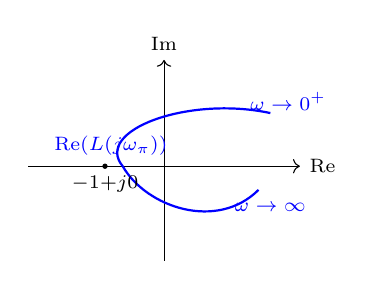
\begin{tikzpicture}[scale=0.75,every node/.style={font=\scriptsize}]
\draw[->] (-2.3,0) -- (2.3,0) node[right]{Re};
\draw[->] (0,-1.6) -- (0,1.8) node[above]{Im};
\draw[thick,blue] (1.8,0.9) .. controls (0.4,1.2) and (-1.2,0.6) .. (-0.7,0) .. controls (-0.3,-0.7) and (0.9,-1.1) .. (1.6,-0.4);
\filldraw (-1,0) circle (1pt) node[below]{$-1{+}j0$};
\node[blue] at (2.1,1.1) {$\omega\to0^+$};
\node[blue] at (1.8,-0.7) {$\omega\to\infty$};
\node[blue] at (-0.9,0.35) {$\mathrm{Re}(L(j\omega_\pi))$};
\end{tikzpicture}
\end{center}

\subsection{Marginea de fază / de amplitudine}
$\omega_t=$ puls. de tăiere: $|L(j\omega_t)|=1$
\begin{keyeq}
$$\gamma=180^\circ+\angle L(j\omega_t)$$
\end{keyeq}
$$\angle L(j\omega)=\sum\left(-\arctan\frac{\omega}{p_i}\right)\ \text{(pt fiecare pol; pol în origine} \to -90^\circ\text{)}$$
\begin{keyeq}
$$|L(j\omega_t)|=1 \iff \prod_i(\omega_t^2+p_i^2)=k^2$$
\end{keyeq}
(pt $L=\dfrac{k}{\prod(s+p_i)}$, $p_i=0$ dacă e integrator) $\Rightarrow$ afli $\omega_t$

$\omega_\pi=$ puls. de fază (calculat la a): $\mathrm{Im}\{L(j\omega_\pi)\}=0$
\begin{keyeq}
$$m_A=\frac1{|L(j\omega_\pi)|}\qquad (m_{A,dB}=-20\lg|L(j\omega_\pi)|)$$
\end{keyeq}
\textbf{Atenție:} $\omega_t\ne\omega_\pi$ în general --- $\omega_t$ e pt $\gamma$ (modul$=1$), $\omega_\pi$ e pt $m_A$ (Im$=0$ / fază$=-180^\circ$).

\section{Locul rădăcinilor}
Poli $p_i$, zerouri $z_j$; $n=$nr.poli, $m=$nr.zerouri. (un singur exercițiu, se rezolvă tot pe rând:)

\textbf{Asimptote:}
\begin{keyeq}
$n-m$ asimptote la număr
$$\theta_k=\frac{180^\circ(2k+1)}{n-m},\ k=0,\dots,n{-}m{-}1$$
$$\sigma_a=\frac{\sum p_i-\sum z_j}{n-m}\ \text{(centrul)}$$
\end{keyeq}

\textbf{Unghi de plecare dintr-un pol complex:}
\begin{keyeq}
$$\varphi_p=180^\circ-\sum\angle(\text{ceilalți poli})+\sum\angle(\text{zerouri})$$
\end{keyeq}
(unghiurile vectorilor de la ceilalți poli/zerouri către polul respectiv; poli scad, zerouri adună)

\textbf{Puncte de rupere (breakaway):} Din $1+G(s)H(s)=0$ izolezi $K(s)$:
\begin{keyeq}
$$K(s)=-\frac1{G(s)H(s)/K}\ \text{(scoți }K\text{ afară)}$$
$$\frac{dK}{ds}=0 \Rightarrow \text{rădăcini reale = puncte de rupere}$$
\end{keyeq}
Dacă există rădăcină reală, o pui înapoi în $K(s)$ ca să afli $K$ acolo. Dacă nu există rădăcină reală $\Rightarrow$ nu există punct de rupere.

\textbf{Intersecția cu axa imaginară:} Două metode echivalente:
(1) Routh: rândul $s^1\to0 \Rightarrow K_{\text{limită}}$, apoi din rândul $s^2$ afli $\omega$.
(2) Substituție directă $s=j\omega$ în $1+G(s)H(s)=0$:
\begin{keyeq}
$\mathrm{Re}=0$ și $\mathrm{Im}=0$ (2 ecuații, 2 necunoscute $\omega,K$)
\end{keyeq}
Dacă rezultă $K>0 \Rightarrow$ locul chiar atinge axa $j\omega$ la acel $\omega$.

\section{Răspuns la intrare sinusoidală}
$x(t)=U\sin(\omega_0t)$ (regim permanent, la ieșirea din $G(s)$):
\begin{keyeq}
$$y(t)=U\,|G(j\omega_0)|\,\sin(\omega_0t+\varphi)$$
\end{keyeq}
$$|G(j\omega_0)|=\frac{|\text{num.}|}{|\text{numit.}|}\ \text{(modul = raport de module, la }s=j\omega_0)$$
$$\varphi=\angle\text{numărător}-\angle\text{numitor}$$

\textbf{Formule suplimentare} (nu de la 5, folosite general):

Buclă închisă (reacție):
\begin{keyeq}
$$G_0(s)=\frac{G(s)}{1+G(s)H(s)}$$
\end{keyeq}
(cea folosită la 1c) $Y(s)=G_0(s)U(s)$; pt reacție unitară $H(s)=1$)

Criteriul Nyquist (general):
\begin{keyeq}
$$Z=N+P$$
\end{keyeq}
$Z=$poli instabili în buclă închisă, $N=$nr. încercuiri ale lui $-1$ (sens trigonometric, pt $\omega:-\infty\to\infty$), $P=$poli instabili în buclă deschisă. $Z=0 \Rightarrow$ stabil în buclă închisă. (Cazul simplu $P=0$: curba nu trebuie să încercuiască $-1$.)

\textbf{Tabel Laplace} (pt fracții simple, 1c):
\begin{center}
\begin{tabular}{@{}ll@{}}
$f(t)$ & $F(s)$\\\hline
$\delta(t)$ & $1$\\
$u(t)$ (treaptă) & $1/s$\\
$t$ (rampă) & $1/s^2$\\
$e^{-at}$ & $1/(s+a)$\\
$\sin(\omega t)$ & $\omega/(s^2{+}\omega^2)$\\
$\cos(\omega t)$ & $s/(s^2{+}\omega^2)$\\
\end{tabular}
\end{center}

\textbf{Reguli generale de reținut}
\begin{itemize}
\item modul unui factor $a+jb$: $\sqrt{a^2+b^2}$ (NU $(a{+}b)^2$!)
\item Unghiul lui $a+jb$, după cadran:\\
\textbf{I} $(a{>}0,b{>}0)$ $\arctan\frac{|b|}{|a|}$\\
\textbf{II} $(a{<}0,b{>}0)$ $180^\circ-\arctan\frac{|b|}{|a|}$\\
\textbf{III} $(a{<}0,b{<}0)$ $-180^\circ+\arctan\frac{|b|}{|a|}$\\
\textbf{IV} $(a{>}0,b{<}0)$ $-\arctan\frac{|b|}{|a|}$
\item $a=0$: unghi $\pm90^\circ$ după semnul lui $b$; $b=0$: unghi $0^\circ$ ($a{>}0$) sau $180^\circ$ ($a{<}0$)
\item $\arctan(x)\to90^\circ$ doar la $x\to\infty$ (limită, niciodată exact la o valoare finită)
\item Pol/zero simplu în origine schimbă faza cu $\mp90^\circ$ constant pe tot graficul
\item La $\omega\to\infty$: faza tinde spre $-90^\circ\times$(nr.poli$-$nr.zerouri)
\item $z_1z_2$: module se înmulțesc, unghiuri se adună. $z_1/z_2$: module se împart, unghiuri se scad.
\item $\omega_t$ (tăiere, $|L|{=}1$) $\ne \omega_\pi$ (fază, Im$=0$) --- frecvențe diferite, nu le confunda
\end{itemize}

\end{multicols}
\end{document}
